\documentclass[a4paper, 10pt]{article}
%\documentclass{article}

\usepackage{stmaryrd}
\usepackage{amsfonts,amsmath,amssymb,mathtools,amsthm}
\usepackage{graphicx}
\usepackage{float}
\usepackage{blindtext}
\usepackage{enumitem}
\usepackage{xcolor}
\usepackage{thmtools}
\usepackage{tikz}
\usetikzlibrary{shapes, arrows, positioning}


\usepackage{graphicx}
%this package is flexible for image insertion
%
\usepackage{alltt}
%this package is suitable for the description of algorithms and computer programs
%
\usepackage{amsmath}
%this package draws mathematical symbols smoothly
%
\usepackage{xcolor}
\definecolor{C0}{HTML}{3182ce}
% \usepackage[breaklinks=true,colorlinks,bookmarks=false,citecolor=C0]{hyperref}
\usepackage[colorlinks=true, linkcolor=C0, citecolor=C0, urlcolor=C0]{hyperref}
\usepackage[margin=2.5cm]{geometry}
% \usepackage[hidelinks, pdftex]{hyperref}
%this package produces hypertext links in the document
\usepackage[round]{natbib}  

\pagenumbering{arabic}
\setcounter{page}{1}
\renewcommand{\thefootnote}{\fnsymbol{footnote}}
\newcommand{\doi}[1]{\href{https://doi.org/#1}{\texttt{https://doi.org/#1}}}

\renewcommand{\P}{\mathbb{P}}
\newcommand{\E}{\mathbb{E}}
\newcommand{\arcosh}{\text{arcosh}}
\newcommand{\arsinh}{\text{arsinh}}
\newcommand{\artanh}{\text{artanh}}

\newcommand{\beq}{\begin{equation}}
\newcommand{\eeq}{\end{equation}}
\newcommand{\bea}{\begin{eqnarray}}
\newcommand{\eea}{\end{eqnarray}}
\newcommand{\beqq}{\begin{equation*}}
\newcommand{\eeqq}{\end{equation*}}
\newcommand{\beaa}{\begin{eqnarray*}}
\newcommand{\eeaa}{\end{eqnarray*}}


\newtheorem{theorem}{Theorem}[section]
\newtheorem{definition}{Definition}[section]
\newtheorem{conjecture}{Conjecture}[section]

\newtheorem{proposition}{Proposition}[section]
\newtheorem{lemma}{Lemma}[section]
\newtheorem{corollary}{Corollary}[section]

\theoremstyle{definition}
\newtheorem{remark}{Remark}[section]
\def\br{\begin{remark}\rm\small}
\def\er{\end{remark}}
\def\bt{\begin{theorem}}
\def\et{\end{theorem}}
\def\bd{\begin{definition}}
\def\ed{\end{definition}}
\def\bp{\begin{proposition}}
\def\ep{\end{proposition}}
\def\bl{\begin{lemma}}
\def\el{\end{lemma}}
\def\bc{\begin{corollary}}
\def\ec{\end{corollary}}
\def\beaq{\begin{eqnarray}}
\def\eeaq{\end{eqnarray}}


\title{Characterisation of optimal sub-Gaussian variance proxy\\ and application to discrete distributions}
\date{}

\begin{document}

\maketitle

%\small
%\textbf {Firstname Lastname, Firstname2 Lastname2, Firstname3 Lastname3}\\[6pt]
%Institution(s) of author(s), address(es) \\ author@somewhere.host\\[6pt]
%Received: date\quad/\quad
%Revised: date\quad/\quad
%Publised online: data

\begin{abstract}
We investigate the problem of characterizing the optimal variance proxy  for random variables whose moment generating function has bounded growth at infinity. Our method is based on a detailed analysis of function variations, leading  to an explicit and practical procedure for computing the optimal variance proxy.  This involves solving a well-defined equation and identifying key critical points. A central result of this work shows that the optimal variance proxy is given by the maximum between the standard variance and a supremum term arising from the function analysis. We apply this approach to discrete random variables, with a particular focus on the case of 3-mass distributions, thus generalizing the well-studied 2-mass or Bernoulli case. In this setting, we derive closed-form solutions for the optimal variance proxy  in several cases, providing explicit characterizations of strict sub-Gaussianity. In particular, we prove that the discrete uniform distribution over 
$N$ points is strictly sub-Gaussian. These findings demonstrate the effectiveness of our method for both theoretical investigations and practical computations involving discrete distributions.
%As an additional contribution, we provide a Python library that collects the main results related to sub-Gaussianity, including our new findings on optimal variance proxies. This resource aims to facilitate further research and practical applications in the study of sub-Gaussian random variables.
\end{abstract}

\tableofcontents

\newpage

\section{Introduction}\label{s:1}
The sub-Gaussian property, first characterized by \citet{Kahane1960PropritsLD} and \citet{buldygin1980sub}, has become a critical tool for understanding the tail behavior of random variables. Since these pioneering works, this property has emerged as a fundamental concept in probability theory due to its profound implications in various mathematical disciplines, such as concentration inequalities \citep{Hoeffding1963, boucheron2003concentration, raginsky2013concentration} and Bayesian statistics \citep{elder2016bayesian, catoni2007pac}. In machine learning, sub-Gaussian tails play a crucial role in bandit algorithms \citep{bubeck2012regret}, in the study of the singular values of random matrices \citep{rudelson2010non}, or in Bayesian neural networks \citep{vladimirova2019understanding, vladimirova2020sub}, to name a few.

\begin{definition}[Sub-Gaussian variables] A random variable \( X \) with finite mean \( \mu = \mathbb{E}[X] \) is \textit{sub-Gaussian} if there exists a constant \( \sigma^2 > 0 \) such that:
\begin{equation}
    \mathbb{E}[\exp(\lambda (X - \mu))] \leq \exp\left(\frac{\lambda^2 \sigma^2}{2}\right), \text{ for all } \lambda \in \mathbb{R}.
    \label{eq:def_sub}
\end{equation}

Such a constant \( \sigma^2 \) is called a \textit{variance proxy} (or \textit{sub-Gaussian norm}), and we say that \( X \) is \(\sigma^2\)-sub-Gaussian. When \( X \) is sub-Gaussian, the primary focus is often on determining the \textit{optimal variance proxy}:
\[
\sigma^2_{\mathrm{opt}}(X) = \inf \left\{ \sigma^2 > 0 \text{ such that } X \text{ is } \sigma^2\text{-sub-Gaussian} \right\}.
\]

For a \(\sigma^2\) sub-Gaussian random variable \(X\), the true variance is always bounded by the variance proxy, i.e. $\operatorname{Var}(X) \leq \sigma^2$, as shown by comparing Taylor expansions of the moment-generating function. When $\sigma^2_{\mathrm{opt}}(X) = \mathrm{Var}(X)$, \(X\) is called \textit{strictly} sub-Gaussian.
\end{definition}

Although extensive research on optimal variance proxy has focused on continuous distributions such as Beta, Dirichlet, and multimodal distributions \citep{marchal2017sub}, as well as Bernoulli, binomial, Kumaraswamy, and triangular distributions \citep{arbel2020strict}, and truncated Gaussian and exponential distributions \citep{barreto2024optimal}, the sub-Gaussianity of discrete distributions remains underexplored, despite their prevalence in modeling count data, binary outcomes, and combinatorial stochastic processes. Our work contributes to filling this gap by developing a general analytic and computational framework for finding the optimal variance proxy and applying it to classes of discrete random variables.


\paragraph{Contributions and outline.}
In this work, we first provide in Section~\ref{sec:charac} a characterization of the optimal sub-Gaussian variance proxy for random variables with bounded moment generating functions, following a general methodology based on function variation analysis. This characterization yields a practical computational procedure via critical point identification and equation solving, enabling explicit computation of the optimal proxy. We then apply this approach with a focus to discrete distributions. We start in Section~\ref{sec:3-mass} with 3-point distributions, both symmetric and asymmetric, extending the classical Bernoulli (2-point) case. In the symmetric setting, we uncover a phase transition: for probabilities $p \geq 1/6$, strict sub-Gaussianity holds, whereas for $p < 1/6$, it does not, and we derive an explicit characterization of the optimal proxy through a pair of solvable equations. In the asymmetric case, we delineate two regimes depending on the relationship between the central mass and the edge probabilities, and in one of these, we provide a closed-form expression for the optimal proxy. Finally, we establish in Section~\ref{sec:uniform} that discrete uniform distributions over $N$ points are strictly sub-Gaussian for all $N$, using a moment-based analysis of the exponential family induced by the log-partition function. These results provide both theoretical insight and numerically tractable tools for assessing sub-Gaussianity in discrete settings.



\section{Characterization of optimal sub-Gaussian variance proxy}\label{sec:charac}

Let $Y$ some real random variable and \( \mu = \mathbb{E}[Y] \). Denote by $M_Y(\lambda):=\ln \left(\mathbb{E}[\exp(\lambda (Y - \mu))]\right)$ the cumulant generating function of the centered random variable $Y-\mu$. 
Define
\beq g_Y(\lambda;\sigma^2):=\frac{1}{2}\lambda^2\sigma^2- M_Y(\lambda)= \frac{1}{2}\lambda^2\sigma^2-\ln \left(\mathbb{E}[\exp(\lambda (Y - \mu))]\right)\eeq
which is a smooth function of $(\lambda,\sigma^2)$.
We have
\beq g'_Y(\lambda;\sigma^2):= \lambda\sigma^2- M_Y'(\lambda)\eeq
Observe that $g_Y(0,\sigma^2)=0=g_Y'(0,\sigma^2)$. Moreover, for $\lambda\neq 0$, the equation $g_Y'(\lambda,\sigma^2)=0$ is equivalent to $\sigma^2=\frac{M_Y'(\lambda)}{\lambda} $. Thus, the system of equations $g_Y(\lambda;\sigma^2)=0$ and $g_Y'(\lambda,\sigma^2)=0$ with $\lambda\neq 0$ is equivalent to  
\beq \sigma^2=\frac{1}{\lambda} M_Y'(\lambda) \text{ and } \lambda\neq 0 \text{ sol. of  } \lambda M_Y'(\lambda)- 2M_Y(\lambda)=0\eeq

Let us define
\beq \mathcal{L}_c^*:=\left\{\lambda_c \in \mathbb{R}^* \,/\,  \lambda_c M_Y'(\lambda_c)- 2M_Y(\lambda_c)=0 \,\, \text{ and }\lambda_c \text{ local min. of } g\left(.,\sigma^2=\frac{ M_Y'(\lambda_c)}{\lambda_c}\right) \right\}\eeq
and define 
\beq \mathcal{S}_c^*=\left\{\frac{M_Y'(\lambda_c)}{\lambda_c}  \,/\, \lambda_c\in \mathcal{L}_c\right\}\eeq
We complement them by defining:
\beq \mathcal{L}_c=\mathcal{L}_c^*\cup\{0\}\,\,, \,\mathcal{S}_c=\mathcal{S}_c^*\cup\{\operatorname{Var}[Y]\}\eeq 

Let us first make the following observation.
\begin{proposition}[Asymptotics at infinity]\label{AsymptInf}If $M_Y(\lambda)\overset{\lambda\to\pm \infty}{=}o(\lambda^2)$ then
\beq \lim_{\lambda\to \pm\infty}g_Y(\lambda;\sigma^2)=+\infty\,,\, \lim_{\lambda\to \pm\infty}g'_Y(\lambda;\sigma^2)=\pm\infty\,,\, \lim_{\lambda\to \pm\infty}g''_Y(\lambda;\sigma^2)=\sigma^2\eeq
and $Y$ is sub-Gaussian. Moreover a sufficient condition is that $Y$ is a bounded random variable.    
\end{proposition}

\begin{proof}The proof is obvious from the definition of $g_Y(\lambda;\sigma^2)=\frac{1}{2}\lambda^2\sigma^2-M_Y(\lambda)$. The sufficient condition is also immediate since if $M$ is a bound for $Y$ then
$|M_Y(\lambda)|\leq \lambda|M+\mu|=o(\lambda^2)$. The fact that $Y$ is sub-Gaussian follows from the fact that there exists $C>0$ such that $|M(\lambda)|\leq C\lambda^2$ for all $\lambda\in \mathbb{R}$. Thus, taking $\sigma^2>C$ immediately gives that $\sigma^2$ is a variance proxy so that $Y$ is sub-Gaussian.
\end{proof}

First, let us prove the following lemma.


%\begin{lemma}\label{LemmaTechnicalGeneral}Assume that $M_Y(\lambda)\overset{\lambda\to \pm\infty}{=}o(\lambda^2)$. If $\sigma_{\mathrm{opt}}^2 > \operatorname{Var}[Y]$ then $\sigma_{\mathrm{opt}}^2$ may only be achieved when $g_Y(.;\sigma_{\mathrm{opt}}^2)$ has at least one point $\lambda_0\in \mathbb{R}^*$ where $g(\lambda_0;\sigma_{\mathrm{opt}}^2)=0=g_Y'(\lambda_0;\sigma_{\mathrm{opt}}^2)$. In other words, $\lambda_0\in \mathcal{L}_c^*$ and $\sigma_{\mathrm{opt}}^2=\frac{M_Y'(\lambda_0)}{\lambda_0}\in \mathcal{S}_c^*$.
%\end{lemma}

%\begin{proof}First, \autoref{AsymptInf} provides control at infinity of the function $g_Y(.;\sigma^2)$ which is positive and locally convex at $\pm \infty$. Then, let us define $\sigma_0^2=\sigma_{\mathrm{opt}}^2 -\frac{1}{2}(\sigma_{\mathrm{opt}}^2-\operatorname{Var}[Y])$. Then observe that for any $\sigma^2\in \left(\sigma_0^2,\sigma_{\mathrm{opt}}^2\right)$, $g(.;\sigma^2)$ is convex non-negative around $\lambda=0$ with $g''(0,\sigma^2)>\sigma_0^2-\operatorname{Var}[Y]>0$. In particular, there exists an interval $(-a,a)$ with $a>0$ where $(\lambda,\sigma^2)\mapsto g(\lambda;\sigma^2)$ is locally positive for any $\lambda\in (-a,a)\setminus\{0\}$ and any $\sigma^2\in \left(\sigma_0^2,\sigma_{\mathrm{opt}}^2\right)$ and such that there exists $A>0$ such that $\sup_{\sigma \in (\sigma_0^2, \sigma_{opt}^2)} \left\{g(-a;\sigma^2),g(a;\sigma^2)\right\} > A$. Thus, for any $\sigma^2\in \left(\sigma_0^2,\sigma_{\mathrm{opt}}^2\right)$, $g(.;\sigma^2)$ has no local minimum except $0$ in $(-a,a)$. Let us consider a local minimum $\lambda_m\neq 0$ (i.e. $|\lambda_m|\geq a$ from the previous discussion) of $g(.;\sigma_{\mathrm{opt}}^2)$ and define $M_m=g(\lambda_m;\sigma_{\mathrm{opt}}^2)$. It is obvious that $M_m$ cannot be strictly negative, otherwise by continuity of $\sigma\to g(\lambda_m;\sigma^2)$, there would exist $\epsilon>0$ such that for any $\sigma^2\in \left(\sigma_{\mathrm{opt}}^2, \sigma_{\mathrm{opt}}^2+\epsilon\right)$: $g(\lambda_m,\sigma^2)<0$ so that $\sigma^2$ would not be a variance proxy in contradiction with the fact that $\sigma_{\mathrm{opt}}^2$ is the optimal variance proxy. Thus we must have $M_m\geq 0$. Assume now by contradiction that there exists $\eta>0$ such that we have all $M_m>\eta$ for all local minima. We shall take $\eta$ sufficiently small so that $\eta<\frac{A}{3}$. In particular, we get that the global minimum of $g(.;\sigma_{\mathrm{opt}}^2)$ on $(-\infty,-a)\cup(a,+\infty)$ is greater than $\eta$. Since $\underset{\lambda\to \pm \infty}{\lim} g(\lambda;\sigma^2)=+\infty$, we may use continuity on a compact set to prove that there exists $\epsilon>0$, with $\epsilon<\frac{1}{2}(\sigma_{\mathrm{opt}}^2-\operatorname{Var}[Y])$ such that the global minimum of $g(.;\sigma^2)$ is greater than $\frac{\eta}{2}$ for any $\sigma^2\in \left(\sigma_{\mathrm{opt}}^2-\epsilon,\sigma_{\mathrm{opt}}^2\right)$. In other words, we may lower $\sigma^2$ from $\sigma_{\mathrm{opt}}^2$ while $g(.;\sigma^2)$ remains non-negative and hence is a variance proxy. This contradicts the fact that $\sigma_{\mathrm{opt}}^2$ is optimal and ends the proof of \autoref{LemmaTechnicalGeneral}.  
%\end{proof} 


The optimal variance proxy is characterized by the following theorem.

\begin{theorem}[Characterization of the optimal variance proxy]\label{GeneralCharac} Let us assume that $M_Y(\lambda)\overset{\lambda\to \pm\infty}{=}o(\lambda^2)$. Then, the optimal variance proxy is characterized by
\beq \sigma_{\mathrm{opt}}^2 = \max\left\{ \operatorname{Var}(Y),\; \sup_{s \in \mathcal{S}_c^*} s \right\} \eeq    
\end{theorem}

\begin{proof}Let us first consider $\sigma^2>\max\left\{ \operatorname{Var}(Y),\; \sup_{s \in \mathcal{S}_c^*} s \right\}$. Then since $\sigma^2>\operatorname{Var}[Y]$, we get that $g(.;\sigma^2)$ is locally convex and non-negative around $\lambda=0$.  Let us consider $\lambda_m(\sigma)\neq 0$ a local minimum of $g(.,\sigma^2)$. For simplicity we shall assume that $\lambda_m(\sigma)>0$ but a similar argument is valid if $\lambda_m(\sigma)<0$. Then we have $\partial_{\sigma}[g(\lambda_m(\sigma);\sigma^2)]= g'(\lambda_m(\sigma);\sigma^2) \partial_\sigma \lambda_m(\sigma) + \lambda_m(\sigma)^2\sigma= \lambda_m(\sigma)^2\sigma>0$. Assume by contradiction that $g(\lambda_m(\sigma);\sigma^2)<0$ then increasing $\sigma$ would increase the value of $g(\lambda_m(\sigma);\sigma^2)$. Since $\partial_{\sigma}[g(\lambda_m(\sigma);\sigma^2)]=\lambda_m(\sigma)^2\sigma>0$ there are only two cases: \begin{itemize}\item $\lambda_m(\sigma)$ remains outside a positive neighborhood of $0$ denoted $(0,\epsilon)$ when we increase $\sigma$ and thus since $\partial_{\sigma}[g(\lambda_m(\sigma);\sigma^2)]>\epsilon^2 \sigma$ there exists a value $\sigma_1>\sigma$ for which $g(\lambda_m(\sigma_1);\sigma_1^2)=0$ which is a contradiction because $\sigma_1^2\in \mathcal{S}_c^*$ so that we should have $\sigma\geq \sigma_1$.
\item $\lambda_m(\sigma)\to 0_+$ when we increase $\sigma$. In this case this is a contradiction because $g(.,\sigma^2)$ is locally positive and convex in a positive neighborhood of $0$. Indeed, $g(.,\sigma^2)$ must reach a positive local maximum on $(0,\lambda_m(\sigma))$ that we denote $\lambda_{\text{max}}(\sigma)$. By Rolle's theorem on $(0,\lambda_{\text{max}}(\sigma))$ and $(\lambda_{\text{max}}(\sigma),\lambda_m(\sigma))$, there exist at least two distinct values $(\lambda_1(\sigma),\lambda_2(\sigma))$ with $0<\lambda_1(\sigma)<\lambda_{\text{max}}(\sigma)<\lambda_2(\sigma)<\lambda_m(\sigma)$ such that $g''(\lambda_1(\sigma);\sigma^2)=g''(\lambda_2(\sigma);\sigma^2)=0$. Since $\lambda_m(\sigma)\to 0_+$, we must also have $\lambda_1(\sigma),\lambda_2(\sigma)\to 0_+$ and hence by continuity $g''(0,\sigma^2)\to 0$. But this is impossible since $g''(0;\sigma^2)=(\sigma^2-\operatorname{Var}[Y])>0$ is a positive, increasing function of $\sigma$. 
\end{itemize}
Thus we conclude that for any $\sigma^2>\max\{\operatorname{Var}[Y],\sup_{s\in \mathcal{S}_c^*}(s)\}$, all local minima of $g(.;\sigma^2)$ are non-negative so that since $\underset{\lambda\to \pm \infty}{\lim} g(\lambda;\sigma^2)=+\infty$, $g(.;\sigma^2)$ is non-negative on $\mathbb{R}$. Hence $\sigma^2$ is a variance proxy and thus $\sigma_{\mathrm{opt}}^2\leq \max\{\operatorname{Var}[Y],\sup_{s\in \mathcal{S}_c^*}(s)\}$.

\medskip

\sloppy{Let us prove the converse inequality and assume that $\sigma_{\mathrm{opt}}^2< \max\{\operatorname{Var}[Y],\sup_{s\in \mathcal{S}_c^*}(s)\}$. It is well-known that $\operatorname{Var}[Y]$ is always a lower bound for the optimal variance proxy, thus the last inequality is only possible if  $\operatorname{Var}[Y]<\sigma_{\mathrm{opt}}^2< \sup_{s\in \mathcal{S}_c^*}(s)$.} Thus, there exists $s_c\in \mathcal{S}_c^*$ such that $\sigma_{\mathrm{opt}}^2<s_c$, i.e. there exists $\lambda_c\in \mathbb{R}^*$ such that $g(\lambda_c;s_c)=g'(\lambda_c;s_c)=0$ and $\lambda_c$ is a local minimum of $g(.;s_c)$. We have from the fact that the dependence of $g$ relatively to $\sigma$ is quadratic that:
\beq g(\lambda_c,\sigma^2)=g(\lambda_c,s_c) +\frac{1}{2}\lambda_c^2 (\sigma^2-s_c)=\frac{1}{2}\lambda_c^2 (\sigma^2-s_c)\eeq
so that $g(\lambda_c,\sigma^2)<0$ when $\sigma^2<s_c$. This implies that $g(.;\sigma^2)$ is no longer non-negative when $\sigma^2<s_c$ so that $\sigma^2$ is not a variance proxy. This contradicts the fact that $\sigma_{\mathrm{opt}}^2<s_c$ is an optimal variance proxy.
\end{proof}


\begin{remark}The main advantage of the characterization of the optimal variance proxy by \autoref{GeneralCharac} is that it gives a numeric way to obtain the optimal variance proxy in practice. Indeed, in order to determine it, one can numerically solve for the equation $\lambda M'(\lambda)-2M(\lambda)=0$. When numeric solutions are found, one should check numerically if $\lambda$ is a local minimum of $g\left(.;\sigma^2=\frac{M'(\lambda)}{\lambda}\right)$ (a sufficient condition being that $g''\left(\lambda;\sigma^2=\frac{M'(\lambda)}{\lambda}\right)>0$). Collecting all solutions, one picks the optimal variance proxy by looking at the maximal values of $\frac{M'(\lambda)}{\lambda}$ that can easily be computed numerically. In practice, such an algorithm is particularly efficient if the number of solutions of $\lambda M'(\lambda)-2M(\lambda)=0$ is low and if one can bound the intervals on which to look for numeric solutions.  
\end{remark}


\begin{remark}
In practice, for a given family of distributions, one should study the elements of $\mathcal{L}_c^*$. If $\mathcal{L}_c^*$ is non empty, one should compare its elements with the corresponding values of $s_c$ to select the optimal variance proxy.
\end{remark}



%\textcolor{orange}{In our case, there are only one non-zero solution when $p_3<4\sqrt{p_1p_2}$ and it is explicit: $2\lambda_0$. In the second regime, we have two non-zero solutions: $2\lambda_0$ and another one on $\mathbb{R}_+$ and we should compare their corresponding values of $s_c$ to decide which gives the optimal variance proxy.}

Another useful result in practice is given in the following general lemma. 

\begin{lemma}[Local minimum when $g_Y''(.;\sigma^2)$ has two positive zeros and $\sigma^2>\text{Var}(Y)$]
\label{LemmaNumber}
Let us define $\sigma_0^2=\sigma_{\mathrm{opt}}^2 -\frac{1}{2}(\sigma_{\mathrm{opt}}^2-\operatorname{Var}[Y])$ and assume that $M_Y(\lambda)\overset{\lambda\to \pm\infty}{=}o(\lambda^2)$ and that for any $\sigma^2\in \left(\operatorname{Var}[Y],+\infty\right)$, $g''(.;\sigma^2)$ has exactly two zeros $(\lambda_1(\sigma),\lambda_2(\sigma))$ such that $0<\lambda_1(\sigma)<\lambda_2(\sigma)$. Then, $g(.;\sigma^2)$ has at most one local minimum on $\mathbb{R}_+^*$. More precisely, if there exists $\sigma_1^2\in \left(\operatorname{Var}[Y],\sigma_0^2\right)$, where  such that $g'(.;\sigma_1^2)$ has a zero on $\mathbb{R}_+^*$, then  $g(.;\sigma^2)$ is strictly positive for $\sigma^2\geq\sigma_1^2$ and $g(.;\sigma^2)$ admits a unique local minimum $\lambda_m(\sigma)$ on $\mathbb{R}_+^*$ located in $\lambda_m(\sigma)\in\left(\lambda_1(\sigma),\lambda_2(\sigma)\right)$ for $\operatorname{Var}[Y]<\sigma^2<\sigma_1^2$. Also, $\lambda_m(\sigma)$ is an increasing function of $\sigma$.\\ 
Then the equations $g(\lambda,\sigma^2)=0=g'(\lambda,\sigma^2)$ have at most one solution on $\mathbb{R}_+^*\times \left(\operatorname{Var}[Y],+\infty\right)$:
\begin{itemize}
    \item if it has no solution, then $g(.;\sigma^2)$ is non-negative on $\mathbb{R}_+$ for any $\sigma^2>\operatorname{Var}[Y]$.
    \item if it has one solution $(\lambda_c,\sigma_c^2)$, then it is necessarily a local minimum and $g(.;\sigma^2)$ is non-negative on $\mathbb{R}_+$ if and only if $\sigma^2\geq \sigma_c^2$. 
\end{itemize}
A similar result is valid on $\mathbb{R}_-^*$. 
\end{lemma}

\begin{proof}The proof follows from the study of variations. Indeed, let us first notice that for any $\sigma^2>\operatorname{Var}[Y]$, we have that $g(.;\sigma^2)$ is locally convex and positive around $\lambda=0$ since $g''(0;\sigma^2)=\sigma^2-\operatorname{Var}[Y]>0$. We also remind that $\underset{\lambda\to \pm \infty}{\lim} g''(\lambda;\sigma^2)=\sigma^2>0$. so that $g(.;\sigma^2)$ is also convex at infinity. Thus, from the assumption that $g''(.;\sigma^2)$ has exactly two zeros $(\lambda_1(\sigma),\lambda_2(\sigma))$ on $\mathbb{R}_+^*$, we conclude either $g''(.;\sigma^2)$ does not change sign at its zeros and in this case, $g(.;\sigma^2)$ is strictly convex on $\mathbb{R}_+^*$ with $g(0;\sigma^2)=0$ so that it is positive and increasing on $\mathbb{R}_+$, thus there is no solution of $g'(.;\sigma^2)=0$ on $\mathbb{R}_+^*$. Or that $g''(.;\sigma^2)$ is necessarily positive on $(0,\lambda_1(\sigma))$, negative on $(\lambda_1(\sigma),\lambda_2(\sigma))$ and positive on $(\lambda_2(\sigma),+\infty)$. Thus, $g'(.;\sigma^2)$ is increasing on $(0,\lambda_1(\sigma))$ and since $g'(0;\sigma^2)$ it is positive on $(0,\lambda_1(\sigma))$. Then, $g'(.;\sigma^2)$ is decreasing on $(\lambda_1(\sigma),\lambda_2(\sigma))$ and then increasing on $(\lambda_2(\sigma),+\infty)$. In particular $g'(.;\sigma^2)$ admits a unique local minimum at $\lambda=\lambda_2(\sigma)$ on $\mathbb{R}_+^*$. Consequently, if $g'(\lambda_2(\sigma);\sigma^2)\geq 0$, then $g(.;\sigma^2)$ is non-negative on $\mathbb{R}_+$ and thus since $g(0;\sigma^2)=0$, we get that $g(.;\sigma^2)$ is non-negative on $\mathbb{R}_+$. Alternatively, if $g'(\lambda_2(\sigma);\sigma^2)<0$, then $g'(.;\sigma^2)$ has exactly two zeros $\lambda_1(\sigma)<\lambda_l(\sigma)<\lambda_r(\sigma)<\lambda_2(\sigma)$ and it is negative on $(\lambda_l(\sigma),\lambda_r(\sigma))$ and positive on $(0,\lambda_l(\sigma))\cup(\lambda_r(\sigma),+\infty)$. Consequently, $g(.;\sigma^2)$ has exactly one local minimum on $\mathbb{R}_+^*$ which is necessarily located in  $(\lambda_1(\sigma),\lambda_2(\sigma))$.
Next, let us observe that:
\beq \partial_\sigma[g'(\lambda_2(\sigma);\sigma^2)]=g''(\lambda_2(\sigma);\sigma^2) \partial_\sigma[\lambda_2(\sigma)]+ 2\sigma\lambda_2(\sigma)=2\sigma\lambda_2(\sigma)>0\eeq
Thus, the local minimum of $g'(.;\sigma^2)$ is an increasing function of $\sigma$, so that if it is null for a value $\sigma_1$, then it is positive for $\sigma>\sigma_1$ and negative for $\sigma<\sigma_1$.
Finally, let us observe that
\beq  \partial_\sigma[g(\lambda_m(\sigma);\sigma^2)]=g'(\lambda_m(\sigma);\sigma^2) \partial_\sigma[\lambda_m(\sigma)]+ \sigma\lambda_m(\sigma)^2=\sigma\lambda_m(\sigma)^2>0\eeq
so that $\lambda_m(\sigma)$ is a increasing function of $\sigma$. Let us denote $(\lambda_c,\sigma_c^2)\in \mathbb{R}_+^*\times \left(\operatorname{Var}[Y],+\infty\right)$ a solution of $g(\lambda,\sigma^2)=0=g'(\lambda,\sigma^2)$, then for $\sigma<\sigma_c$, we have $g(\lambda_m(\sigma);\sigma^2)<0$ while for $\sigma>\sigma_c$, we have $g(\lambda_m(\sigma);\sigma^2)>0$. Since $g(.;\sigma^2)$ has only a unique local minimum $\lambda_m(\sigma)$ and a local maximum on $\mathbb{R}_+^*$ which is always strictly positive, we conclude that we cannot have another solution of $g(\lambda,\sigma^2)=0=g'(\lambda,\sigma^2)$ with $\lambda\in \mathbb{R}_+^*$. When there is no solution, we have $g(\lambda_m(\sigma);\sigma^2)>0$ so that $g(.;\sigma^2)$ is non-negative on $\mathbb{R}_+^*$. When we have a unique solution $(\lambda_c,\sigma_c^2)$, then $g(\lambda_m(\sigma);\sigma^2)>0$ for $\sigma>\sigma_c$, $g(\lambda_m(\sigma_c);\sigma_c^2)=0$ and $g(\lambda_m(\sigma);\sigma^2)<0$ for $\sigma<\sigma_c$ concluding the proof. 
\end{proof}

\begin{remark} The cases where $g''$ has no or one zero on $\mathbb{R}_+^*$ are trivial for $\sigma^2\geq \operatorname{Var}[Y]$. Indeed, if $g''(.;\sigma^2)$ has no zero on $\mathbb{R}_+^*$, then it is strictly convex on $\mathbb{R}_+^*$ and since $g(0;\sigma^2)=g'(0;\sigma^2)=0$, $g(.;\sigma^2)$ is positive on $\mathbb{R}_+^*$. If $g''(.;\sigma^2)$ has a unique zero on $\mathbb{R}_+^*$, then it cannot change sign at this zero, because $g''(0;\sigma^2)=\sigma^2-\operatorname{Var}[Y]\geq 0$ and $\underset{\lambda\to +\infty}{\lim}g''(\lambda;\sigma^2)=\sigma^2>0$. Hence, we conclude similarly that $g(.;\sigma^2)$ is positive on $\mathbb{R}_+^*$. 
\end{remark}

We may complement \autoref{LemmaNumber} with another lemma regarding the situation when $\sigma<\sigma_{\mathrm{opt}}$.

\begin{lemma}[Local minimum when $g_Y''(.;\sigma^2)$ has two positive zeros and $\sigma^2<\operatorname{Var}(Y)$]\label{LemmaNumber2}
Assume that $M_Y(\lambda)\overset{\lambda\to \pm\infty}{=}o(\lambda^2)$ and that for any $\sigma^2\in \left(0,\operatorname{Var}[Y]\right)$, $g''(.;\sigma^2)$ has exactly two zeros $(\lambda_1(\sigma),\lambda_2(\sigma))$ such that $0<\lambda_1(\sigma)<\lambda_2(\sigma)$. Then, there is no solution to the set of equations $g_Y(\lambda;\sigma^2)=0=g_Y'(\lambda;\sigma^2)$ with $\lambda>0$ and $\sigma^2\in \left(0,\operatorname{Var}[Y]\right)$.\\
A similar result holds on $\mathbb{R}_-^*$.
\end{lemma}

\begin{proof}For any $\sigma^2<\operatorname{Var}[Y]$, we have that $g_Y(\lambda\sigma^2)=(\sigma^2-\operatorname{Var}[Y])\lambda^2+o(\lambda^2)$ when $\lambda\to 0_+$. Thus, $g(.;\sigma^2)$ is locally concave and negative around $\lambda=0_+$. Since  $M_Y(\lambda)\overset{\lambda\to \pm\infty}{=}o(\lambda^2)$, we know that $g_Y(.;\sigma^2)$ is locally convex and positive when $\lambda\to +\infty$. Since $g_Y''(.;\sigma^2)$ is assumed to have exactly two positive zeros $\lambda_1(\sigma)<\lambda_2(\sigma)$, we may only have the following cases:
\begin{itemize}
    \item $g''_Y(.;\sigma^2)$ is negative on $(0,\lambda_1(\sigma))$ and changes sign at $\lambda_1(\sigma)$. Thus, it is positive on $(\lambda_1(\sigma),\lambda_2(\sigma))$ and cannot change sign at $\lambda_2(\sigma)$ to remain positive at $+\infty$. Hence, $g''_Y(.;\sigma^2)$ is positive on $(\lambda_1(\sigma),\lambda_2(\sigma))\cup (\lambda_2(\sigma),+\infty)$. Consequently, $g'_Y(.;\sigma^2)$ is decreasing on $(0,\lambda_1(\sigma))$ and increasing on $(\lambda_1(\sigma),+\infty)$. Since $g'_Y(0;\sigma^2)$, we have $g'_Y(\lambda_1(\sigma);\sigma^2)<0$ and since $g'_Y(+\infty;\sigma^2)=+\infty$, $g'_Y$ has only one zero $\lambda_0(\sigma)$ on $\mathbb{R}_+^*$ that satisfies $\lambda_0(\sigma)>\lambda_1(\sigma)$. Moreover, $g'_Y(.;\sigma^2)$ is negative on $(0,\lambda_0(\sigma))$ and positive on $(\lambda_0(\sigma),+\infty)$. Hence, $g_Y(.;\sigma^2)$ is decreasing on $(0,\lambda_0(\sigma))$ and increasing on $(\lambda_1(\sigma),+\infty)$. Since $g_Y(0;\sigma^2)=0$ and $g_Y(+\infty;\sigma^2)=+\infty$, $g_Y$ admits a unique zero $\lambda_*(\sigma)$ on $\mathbb{R}_+^*$ and we have $\lambda_*(\sigma)>\lambda_0(\sigma)$. Hence, there are no simultaneous solutions to $g_Y(\lambda;\sigma^2)=0=g_Y'(\lambda;\sigma^2)$ with $\lambda>0$.
    \item $g''_Y(.;\sigma^2)$ is negative on $(0,\lambda_1(\sigma))$ and does not change sign at $\lambda_1(\sigma)$ so it is negative on $(0,\lambda_2(\sigma))$. In order to be positive at $\lambda\to +\infty$, $g_Y''(.;\sigma^2)$ must change sign at $\lambda=\lambda_2(\sigma)$. Thus, $g_Y'(.;\sigma^2)$ is decreasing on $(0,\lambda_2(\sigma))$ and increasing on $(\lambda_2(\sigma),+\infty)$. Since $g_Y'(0;\sigma^2)=0$ and $g_Y'(+\infty;\sigma^2)=+\infty$, $g_Y'(.;\sigma^2)$ admits a unique zero $\lambda_0(\sigma)$ on $\mathbb{R}_+^*$ and it satisfies $\lambda_0(\sigma)>\lambda_2(\sigma)$. Moreover, $g_Y'(.;\sigma^2)$ is negative on $(0,\lambda_0(\sigma))$ and positive on $(\lambda_0(\sigma),+\infty)$. Since $g_Y(0;\sigma^2)=0$ and $g_Y(+\infty;\sigma^2)=+\infty$, $g_Y(.,\sigma^2)$ is decreasing and negative on $(0,\lambda_0(\sigma))$ and increasing on $(\lambda_0(\sigma),+\infty)$. Hence, $g_Y(.;\sigma^2)$ admits a unique zero $\lambda_*(\sigma)$ on $\mathbb{R}_+^*$ and we have $\lambda_*(\sigma)>\lambda_0(\sigma)$. Hence, there are no simultaneous solutions to $g_Y(\lambda;\sigma^2)=0=g_Y'(\lambda;\sigma^2)$ with $\lambda>0$.
\end{itemize}
\end{proof}


\section{Application to 3-mass distributions}\label{sec:3-mass}
\subsection{Symmetric case of 3-mass distributions}\label{subsec;symmthreepoints}
\subsubsection{Notations and main results}
Let $X$ be a random variable such that $X(\Omega)=\{-a,0,a\}$ and 
\begin{equation}
    \P(X=-a)=p\,,\, \P(X=0)=1-2p\,,\, \P(X=a)=p
\end{equation}
where $p\in \left( 0,\frac{1}{2}\right)$ and $a>0$. We may define $Y=\frac{1}{a}X$ and use the fact that $\sigma_{\mathrm{opt}}[Y]=a \sigma_{\mathrm{opt}}[X]$. Thus, we may restrict to $a=1$. We have
\beq \mu:=\E[Y]=0\,\,,\,\, \sigma^2:=\operatorname{Var}[Y]=2p\eeq
For any $\sigma>0$, we have that $\sigma$ is a variance proxy of $Y$ if and only if
\beq \E\left[e^{\lambda (Y-\mu)}\right]=p e^{\lambda }+ pe^{-\lambda } +1-2p\leq e^{\frac{\lambda^2\sigma^2}{2}} \,\, ,\,\, \forall \, \lambda\in \mathbb{R}\eeq
This inequality is equivalent to
\beq g_{\sigma,p}(\lambda):=\frac{\lambda^2\sigma^2}{2}-\ln( 2p\cosh \lambda +1-2p)\geq 0 \,\,,\,\,  \forall \, \lambda\in \mathbb{R}\eeq
Since $g_{\sigma,p}$ is an even function of $\lambda$, this is equivalent to 
\beq g_{\sigma,p}(\lambda):=\frac{\lambda^2\sigma^2}{2}-\ln( 2p\cosh \lambda +1-2p)\geq 0 \,\,,\,\,  \forall \, \lambda\in \mathbb{R}_+\eeq
The general theory implies that $\operatorname{Var}[Y]=2p$ is a lower bound for the optimal variance proxy. In other words, if $\sigma<\sqrt{2p}$ then $\sigma$ is not a variance proxy. Consequently, we shall only consider $\sigma\geq \sqrt{2p}$ in the following proof.
\medskip

The function $g_{\sigma,p}$ is obviously a smooth function of $(\lambda,\sigma,p)$ and we have
\bea g^{'}_{\sigma,p}(\lambda)&=&\lambda \sigma^2 -\frac{2p\sinh \lambda }{2p\cosh \lambda +1-2p}\cr 
g^{(2)}_{\sigma,p}(\lambda)&=&\sigma^2+\frac{2p\left(2p\cosh \lambda -\cosh \lambda -2p)\right)}{(2p\cosh \lambda +1-2p)^2}\cr
g^{(3)}_{\sigma,p}(\lambda)&=&\frac{2p\sinh \lambda\left(4p^2+4p-1+2p(1-2p)\cosh \lambda\right) }{(2p\cosh \lambda +1-2p)^3}
\eea
Let us now observe that 
\beq \forall \, \lambda\in \mathbb{R} \,:\,N_{p}(\lambda):=4p^2+4p-1+2p(1-2p)\cosh \lambda \geq 1.\eeq
and $g^{(3)}_{\sigma,p}(0)=0$. Thus, $g^{(3)}_{\sigma,p}$ and $N_{p}$ have the same sign on $\mathbb{R}_+$. Since $N_{p}'(\lambda)=2p(1-2p)\sinh \lambda$, we get that $N_{p}$ is a strictly increasing function on $\mathbb{R}_+$. Since $N_{p}(0)=6p-1$, we get two distinct cases:
\begin{itemize}
    \item $p\geq \frac{1}{6}$: In this case $N_{p}$ is a positive function on $\mathbb{R}_+$ and so is $g^{(3)}_{\sigma,p}$. It follows that $g_{\sigma,p}^{(2)}$ is a strictly increasing function on $\mathbb{R}_+$. Since $g^{(2)}_{\sigma,p}(0)=\sigma^2-2p\geq0$, it we conclude that $g^{(2)}_{\sigma,p}$ is positive  on $\mathbb{R}_+$. Thus $g^{'}_{\sigma,p}$ is a strictly increasing function on $\mathbb{R}_+$. Furthermore, since $g_{\sigma,p}'(0)=0$ we end up with the fact that $g_{\sigma,p}'$ is a positive function on $\mathbb{R}_+$ and therefore $g_{\sigma,p}$ is an increasing function on $\mathbb{R}_+$. Finally, since $g_{\sigma,p}(0)=0$ we conclude that $g_{\sigma,p}$ is positive on $\mathbb{R}_+$ so that $\sigma$ is a variance proxy. This argument is valid for any $\sigma^2\geq \operatorname{Var}[Y]=2p$ so that $\sigma^2_{opt}[Y]=\operatorname{Var}[Y]=2p$, i.e. {$Y$ is strictly sub-Gaussian}.
    \item $p<\frac{1}{6}$: In this case $N_{p}(0)<0$, and $N_{p}$ is increasing on $\mathbb{R}_+$, tending to $+\infty$ when $\lambda\to +\infty$. Thus since $N_{p}$ is a smooth function, there exists a unique $\lambda_0=\arcosh\left(\frac{1-4p-4p^2}{2p(1-2p)}\right)>0$ such that $N_{p}(\lambda_0)=0$. Moreover $N_{p}$ is strictly negative on $(0,\lambda_0)$ and strictly positive on $(\lambda_0,+\infty)$. These properties immediately extend to $g_{\sigma,p}^{(3)}$. Consequently, $g_{\sigma,p}^{(2)}$ is strictly decreasing on $(0,\lambda_0)$ and strictly increasing on $(\lambda_0,+\infty)$. Additionally, we have $g_{\sigma,p}^{(2)}(0)=\sigma^2-2p\geq 0$ and $g_{\sigma,p}^{(2)}(\lambda_0)=\sigma^2-\frac{(1-2p)^2}{4(1-4p)}$ and $g_{\sigma,p}^{(2)}(+\infty)=\sigma^2>0$. Note that if $\sigma^2\geq \frac{(1-2p)^2}{4(1-4p)}$ then $g^{(2)}_{\sigma,p}$ is positive on $\mathbb{R}_+$ and then it is straightforward to prove that $\sigma$ is a variance proxy using the same final steps as the case $p\geq\frac{1}{6}$. Thus, we conclude that $\sigma_{\text{up}}(p):=\frac{(1-2p)^2}{4(1-4p)}$ {is an upper bound for the optimal variance proxy of $Y$}. Note also that $\sigma=2p$ is no longer a variance proxy because $g^{'}_{\sigma,p}$ would become strictly decreasing on $(0,\lambda_0)$ and thus strictly negative on this interval (because $g^{'}_{\sigma,p}(0)=0$) and so $g_{\sigma,p}$ would be negative on $(0,\lambda_0)$ (again because $g_{\sigma,p}(0)=0)$. This proves that {for $p<\frac{1}{6}$, $Y$ is not strictly sub-Gaussian}. 
\end{itemize}

Let us be more precise in the case $p<\frac{1}{6}$. As mentioned above, we shall now only consider $2p<\sigma^2<\frac{(1-2p)^2}{4(1-4p)}$. The previous analysis implies that there exists a unique pair $(\lambda_1,\lambda_2)$ such that $0<\lambda_1<\lambda_0<\lambda_2$ and $g_{\sigma,p}^{(2)}(\lambda_1)=g_{\sigma,p}^{(2)}(\lambda_2)=0$. Moreover, $g_{\sigma,p}^{(2)}$ is strictly positive on $(0,\lambda_1)\cup(\lambda_2,+\infty)$ and strictly negative on $(\lambda_1,\lambda_2)$. 
Note that we have explicitly:
\bea \lambda_1&:=&\arcosh\left(  \frac{(1-2p)(1-2\sigma^2)-\sqrt{(1-2p)^2-4(1-4p)\sigma^2 } }{4p\sigma^2}\right)\cr
\lambda_2&:=&\arcosh\left(  \frac{(1-2p)(1-2\sigma^2)+\sqrt{(1-2p)^2-4(1-4p)\sigma^2 } }{4p\sigma^2}\right)
\eea
This implies that $g_{\sigma,p}'$ is increasing on $(0,\lambda_1)$, then decreasing on $(\lambda_1,\lambda_2)$ and finally increasing on $(\lambda_2,+\infty)$. Since $g_{\sigma,p}'(0)=0$ and $g_{\sigma,p}'(+\infty)=+\infty$, the sign of $g_{\sigma,p}'$ is determined by the sign of $g_{\sigma,p}'(\lambda_2)$. Note also that a straightforward computation implies that $g_{\sigma,p}'(\lambda_0)=\sigma^2 \lambda_0\sqrt{(1-6p)(1+2p)(1-4p)}>0$. There are only two cases:
\begin{itemize}
\item $g_{\sigma,p}'(\lambda_2)\geq 0$: In this case $g_{\sigma,p}'$ is positive on $\mathbb{R}_+$ so that $g_{\sigma,p}$ is positive on $\mathbb{R}_+$ and thus $\sigma$ is a variance proxy. Thus an upper bound is $\sigma^2_{\text{up}_2}$ that is the unique solution in $\left(2p,\frac{(1-2p)^2}{4(1-4p)}\right)$ of 
\beq \sigma^2_{\text{up2}}=\frac{2p\sinh\lambda_2(\sigma_{\text{up}_2})}{\lambda_2(\sigma_{\text{up}_2}) (1+2p\cosh \lambda_2(\sigma_{\text{up}_2})-2p) }\eeq
where $\lambda_2(x)=\arcosh\left(  \frac{(1-2p)(1-2x^2)+\sqrt{(1-2p)^2-4(1-4p)x^2 } }{4px^2}\right)$
\item $g_{\sigma,p}'(\lambda_2)<0$: In this case, there exists a unique pair $(\lambda_3,\lambda_4)$ such that $\lambda_0<\lambda_3<\lambda_2<\lambda_4$ and $g_{\sigma,p}'(\lambda_3)=g_{\sigma,p}'(\lambda_4)=0$. Moreover, $g_{\sigma,p}'$ is positive on $(0,\lambda_3)\cup(\lambda_4,+\infty)$ and negative on $(\lambda_3,\lambda_4)$. This implies that $g_{\sigma,p}$ increases on $(0,\lambda_3)$, then decreases on $(\lambda_3,\lambda_4)$ and finally increases on $(\lambda_4,+\infty)$. In particular, since $g_{\sigma,p}(0)=0$ and $g_{\sigma,p}(+\infty)=+\infty$, $g_{\sigma,p}$ has only one local maximum $\lambda_3$ and one local minimum $\lambda_4$ on $(0,+\infty)$. Moreover, these local extremum satisfy $0<\lambda_3<\lambda_0<\lambda_4$ and $g_{\sigma,p}(\lambda_3)>0$. Eventually the sign of $g_{\sigma,p}(\lambda_4)$ determines if $\sigma$ is a variance proxy or not. Since $g_{\sigma,p}(\lambda_4)$ is a smooth function of $\sigma$, the critical case corresponding to $\sigma_{\mathrm{opt}}$ may happen only when $g_{\sigma_{\mathrm{opt}},p}(\lambda_4)=0$. Since we know that this critical case is achieved on $\left(2p,\frac{1-4p+4p^2}{4(1-4p)}\right)$ we conclude with the following statement.
\end{itemize}

\begin{proposition}\label{Propplower16} Let $p\in \left(0,\frac{1}{6}\right)$, then the optimal variance proxy $\sigma_{\mathrm{opt}}^2$ is the unique solution of 
\bea 0&=&g_{\sigma_{\mathrm{opt}},p}(\lambda_c)=\frac{\lambda_c^2\sigma_{\mathrm{opt}}^2}{2}-\ln( 2p\cosh \lambda_c +1-2p)\cr
0&=&g^{'}_{\sigma_{\mathrm{opt}},p}(\lambda_c)=\lambda_c \sigma_{\mathrm{opt}}^2 -\frac{2p\sinh \lambda_c }{2p\cosh \lambda_c +1-2p}
\eea
where $\lambda_c\in (\lambda_0,+\infty)$ is the unique solution in $\lambda_c$, with $\lambda_0=\arcosh\left(\frac{1-4p-4p^2}{2p(1-2p)}\right)>0$. The optimal variance proxy satisfies $2p<\sigma_{\mathrm{opt}}^2<\frac{(1-2p)^2}{4(1-4p)}$.
\end{proposition}

\begin{figure}[H]
\centering
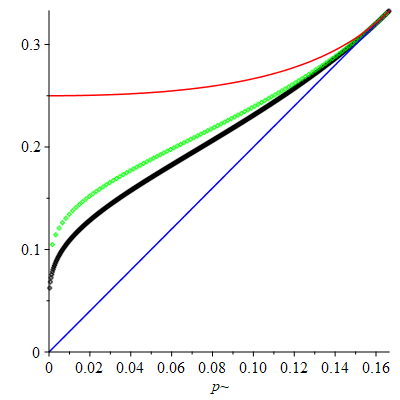
\includegraphics[width=8cm]{NumericPlot.png}
\caption{Numeric plot of the optimal variance proxy (black dots) for $0<p<\frac{1}{6}$. In blue is the variance $2p$ and in red is the upper bound $\sigma_{\text{up}_2}(p):=\frac{(1-2p)^2}{4(1-4p)}$. In green is the numeric evaluation of the upper bound $\sigma_{\text{up2}}^2$.}
\label{241029160152}
\end{figure}


\subsubsection{Refinements and comments}
It is easy to express $\sigma_{\mathrm{opt}}^2$ in terms of $\lambda_c$. It gives a complicated equation for $\lambda_c$:
    \beq p\lambda_c \sinh \lambda_c -(1-2p+2p\cosh \lambda_c)\ln (1-2p+2p\cosh \lambda_c)=0\eeq 
    which to my knowledge does not admit explicit formulas but can easily be solved (and there is a unique zero on $(\lambda_0,+\infty)$) numerically. The knowledge of $\lambda_c$ implies then that
    \beq \sigma_{\mathrm{opt}}^2=\frac{2p\sinh \lambda_c }{\lambda_c(2p \cosh \lambda_c +1-2p)} \eeq 

\medskip

The most important point is that we have two regimes which is quite unusual. For $p\in \big[\frac{1}{6},\frac{1}{2}\big)$ we have strict-sub-Gaussianity while for $p\in \left(0,\frac{1}{6}\right)$ we no longer have sub-Gaussianity. This fact can be proved and also we can characterize the optimal variance proxy has the unique solution of a couple of equations. This can be solved numerically since we also have a lower bound (variance) and two upper bounds: one is simple but no so precise and the second one requires to solve numerically an explicit equation but is more precise. I think it gives a good story to tell. 

\medskip

Other cases that we may look after:
\begin{itemize}
    \item The case where we have $X(\Omega)=\{-a,0,a\}$ but with different probability in $-a$ and $a$ (i.e. $\P(X=-a)=p_1$ and $\P(X=a)=p_2$). In this case, we can also scale out $a$ so that we get two parameters. Be careful that the mean is no longer $0$ in this case. We get a compact space of parameters that is 2 dimensional so that we can at least give a plot of $\sigma_{\mathrm{opt}}^2(p_1,p_2)$ as a $3D$ picture. Maybe the analysis can be carried out up to some extent. In particular the strict sub-Gaussianity cases should be characterized.
    \item The generic case. After translation and dilation, we can take $X(\Omega)=\{-1,0,1+\epsilon\}$ with $\epsilon\in (-1,+\infty)$. In this case, we have $3$ parameters: $p_1$,$p_2$ and $\epsilon$. This complicates the numeric plots. The exact analysis seems also difficult but maybe we can find some conditions where to have strict-sub-Gaussianity. 
\end{itemize}

\subsection{Asymmetric case of 3-mass distributions}\label{subsec;asymmthreepoints}

Let $X$ be a random variable such that $X(\Omega)=\{-a,0,a\}$ and 
\begin{equation}
    \P(X=-a)=p_1\,,\, \P(X=0)=p_3 = 1-p_1-p_2\,,\, \P(X=a)=p_2
\end{equation}
where $p_1, p_2\in \left( 0,1\right) \text{ and since } p_3=0$ corresponds to two masses case  we will consider $p_3 > 0$ and $a>0$. We may define $Y=\frac{1}{a}X$ and use the fact that $\sigma_{\mathrm{opt}}[X]=a \sigma_{\mathrm{opt}}[X]$. Thus, we may restrict to $a=1$. We also may assume $p_2 \geq p_1$ and by considering $Y=-X$. We have
\beq \mu:=\E[Y]=-p_1+p_2 \geq 0\,\,,\,\, \sigma^2:=\operatorname{Var}[Y]=p_1+p_2-(-p_1+p_2)^2\eeq
For any $\sigma>0$, we have that $\sigma$ is a variance proxy of $Y$ if and only if
\beq \E\left[e^{\lambda Y}\right]=p_1 e^{-\lambda }+ p_2e^{\lambda } +1-p_1-p_2\leq e^{(\frac{\lambda^2\sigma^2}{2}+\lambda \mu)} \,\, ,\,\, \forall \, \lambda\in \mathbb{R}\eeq
This inequality is equivalent to
\beq g_{\sigma,p}(\lambda):=\frac{\lambda^2\sigma^2}{2}-\ln(u_{0;p_1, p_2}(\lambda))+\lambda \mu \geq 0 \,\,,\,\,  \forall \, \lambda\in \mathbb{R}\eeq
With  $u_{0;p_1, p_2}(\lambda) := p_1e^{-\lambda}+p_2e^{\lambda}+1-p_1-p_2$ a smooth function and  $u_{0;p_1, p_2}(\lambda) > 0 \text{ , } \forall \lambda \in \mathbb{R}$. Thus the function $g_{\sigma,p}$ is a smooth function of $(\lambda,\sigma,p)$. For convenience we will use simply $u_0(\lambda)$ and we define
\beq u_{i}(\lambda)=u_{i-1}'(\lambda),   \  i  \in \{1,2,3\} \,\,,\,\,  \forall \, \lambda\in \mathbb{R}\eeq
We have $u_1(\lambda) = - p_1e^{-\lambda} + p_2e^{\lambda}$ and we observe that $u_2(\lambda) = u_0(\lambda)-p_3$, $u_3(\lambda) = u_1(\lambda)$ and $u_1^2(\lambda)=(u_0(\lambda)-p_3)^2-4p_1p_2$ for all $\lambda \in \mathbb{R}$ \\
%Since $g_{\sigma,p}$ is an even function of $\lambda$, this is equivalent to 
%\beq g_{\sigma,p}(\lambda):=\frac{\lambda^2\sigma^2}{2}-\ln( 2p\cosh \lambda +1-2p)\geq 0 \,\,,\,\,  %\forall \, \lambda\in \mathbb{R}_+\eeq
The general theory implies that $\operatorname{Var}[Y]=p_1+p_2-(-p_1+p_2)^2$ is a lower bound for the optimal variance proxy. In other words, if $\sigma<\sqrt{p_1+p_2-(-p_1+p_2)^2}$ then $\sigma$ is not a variance proxy. Consequently, we shall only consider $\sigma \geq\sqrt{p_1+p_2-(-p_1+p_2)^2}$ in the following proof.
%\medskip

The function $g_{\sigma,p}$ a smooth function of $(\lambda,\sigma,p)$ and its first derivatives can be expressed as:

\bea g^{'}_{\sigma,p}(\lambda)&=&\lambda \sigma^2 -\frac{u_1(\lambda)}{u_0(\lambda)} + \mu \cr 
g^{(2)}_{\sigma,p}(\lambda)&=& \sigma^2-\frac{u_0(\lambda)p_3-p_3^2+4p_1p_2}{u_0(\lambda)^2}\cr
g^{(3)}_{p}(\lambda)&=& u_1(\lambda)\frac{p_3u_0(\lambda)+8p_1p_2-2p_3^2}{u_0(\lambda)^3}
\eea
Note in particular that $g^{(3)}_{p}$ does not depend on $\sigma$. Moreover, $g^{(3)}_{p}$ can be written as
\beq\label{g3} g^{(3)}_{p}(\lambda) = \frac{u_1(\lambda)N_{p_1,p_2}(\lambda)}{u_0(\lambda)^3} \eeq
where $N_{p_1,p_2}(\lambda) := p_3u_0(\lambda)+8p_1p_2-2p_3^2$. Observe that $u_0(\lambda)$ is strictly positive on $\mathbb{R}$. Therefore, the function $g^{(3)}$ and $N_{p_1, p_2} u_1$ share the same sign. We know that $u_1$ changes sign at $\lambda_0 := -\frac{1}{2}\ln(\frac{p_2}{p_1})$ assuming that $p_2\geq p_1$ we have $\lambda_0 \leq 0$. Hence, to determine the sign of $g^{(3)}$, it remains to analyze the sign of $N_{p_1, p_2}$. For this purpose, it is sufficient to  study the sign of the polynomial
\bea P(X) :=p_2p_3X^2+(8p_1p_2-p_3^2)X+p_3p_1, \text{where}\  X = e^{\lambda} > 0.\eea 
To determine the sign of $P(X)$, we compute its discriminant:
\bea \Delta = (p_3^2)^2 - 20p_1p_2(p_3)^2 + 64p_1^2p_2^2= (p_3^2-4p_1p_2)(p_3^2-16p_1p_2) \eea 
and it gives two different regimes that we shall study separately. In order to perform the study, we shall prove the following lemma.


\subsubsection{The case $p_3\leq 4\sqrt{p_1p_2}$}
In this case, we shall prove the following theorem.
\begin{theorem}[Explicit value of the optimal variance proxy for $p_3\leq 4\sqrt{p_1p_2}$]\label{TheoRegime1} When $p_3\leq 4\sqrt{p_1p_2}$, the optimal variance proxy is given by
\beq \sigma_{\mathrm{opt}}^2= \frac{2(p_2-p_1)}{\ln \frac{p_2}{p_1}}.\eeq
\end{theorem}

\begin{proof}Let us first observe that $\left(2\lambda_0,\sigma_{\mathrm{opt}}^2\right)=\left(-\ln\frac{p_2}{p_1},\sigma_{\mathrm{opt}}^2\right)$ is a solution $(\lambda,\sigma^2)$ of the system of equations
\beq g_{\sigma,p}(\lambda)=0 \text{ and } g^{'}_{\sigma,p}(\lambda) = 0\eeq
Moreover, the case $p_3\leq 4\sqrt{p_1p_2}$ is equivalent to the fact that $\Delta\leq 0$ or $\Delta>0$ with $P$ admitting two strictly negative roots (the sum of roots ($X_1,X_2)$ is $X_1+X_2 = \frac{p_3^2-8p_1p_2}{p_2p_3} < 0$ and the product of roots $X_1 X_2 = \frac{p_1}{p_2}>0$). Thus, the function $N_{p_1,p_2}$ is strictly positive on $\mathbb{R}$. Consequently, $g^{(3)}_{\sigma,p}$ and $u_1(\lambda)$ share the same sign and hence $g_{\sigma,p}^{(3)}$ is strictly negative on $(-\infty,\lambda_0)$ and strictly positive on $(\lambda_{0}, +\infty)$. Furthermore, since $\lim_{\lambda\to \pm \infty} g^{(2)}_{\sigma, p}(\lambda)=\sigma^2$, it follows that $\lambda_0$ is a global minimum of $g^{(2)}_{\sigma, p}$ with value $g^{(2)}_{\sigma,p}(\lambda_{0})=\sigma^2-\frac{2\sqrt{p_1p_2}}{p_3+2\sqrt{p_1p_2}}$. If $\sigma^2\geq\frac{2\sqrt{p_1p_2}}{p_3+2\sqrt{p_1p_2}}$ , then $g^{(2)}_{\sigma,p}$ is non-negative on $\mathbb{R}$ and so $g'_{\sigma,p}$ is a strictly increasing function. Since $g'_{\sigma,p}(0)=0$, $g'_{\sigma,p}$ is negative on $\mathbb{R}_-$ and positive on $\mathbb{R}_+$ and finally $g_{\sigma,p}$ has a global minimum at $\lambda=0$ which is precisely null so it is positive and $\sigma^2$ is a variance proxy. This gives that $\frac{2\sqrt{p_1p_2}}{p_3+2\sqrt{p_1p_2}}$ is an upper bound for the optimal variance proxy. 

On the contrary, if $\sigma^2<\frac{2\sqrt{p_1p_2}}{p_3+2\sqrt{p_1p_2}}$, then $g^{(2)}_{\sigma, p}$ has two distinct zeros $(\lambda_1(\sigma),\lambda_2(\sigma))$ such that $\lambda_1(\sigma)<\lambda_0<\lambda_2(\sigma)\leq 0$. Moreover, since $g_{\sigma,p}''(.;\sigma^2)$ is positive on $\mathbb{R}_+^*$, we get that $g_{\sigma,p}(.;\sigma^2)$ is always positive on $\mathbb{R}_+^*$ for any $\sigma^2\in \left(\operatorname{Var}[Y],\frac{2\sqrt{p_1p_2}}{p_3+2\sqrt{p_1p_2}} \right) $. Since, we have observed that the equations $g_{\sigma,p}(\lambda,\sigma^2)=0=g_{\sigma,p}'(\lambda,\sigma^2)$ admits $\left(2\lambda_0,\frac{2(p_2-p_1)}{\ln \frac{p_2}{p_1}}\right)\in \mathbb{R}_-^*\times \left(\operatorname{Var}[Y],+\infty\right)$ as solution, application of \autoref{LemmaNumber} on $\mathbb{R}_-^*$ implies that $g_{\sigma,p}(.;\sigma^2)$ is non-negative on $\mathbb{R}_-$ if and only if $\sigma^2\geq \frac{2(p_2-p_1)}{\ln \frac{p_2}{p_1}} $. Thus the optimal variance proxy in this case is $\sigma_{\mathrm{opt}}^2= \frac{2(p_2-p_1)}{\ln \frac{p_2}{p_1}}$ . 

\end{proof}

\autoref{TheoRegime1} implies the following corollary.

\begin{corollary}\label{Strictsub-GaussianityRegime1} For $p_3\leq 4\sqrt{p_1p_2}$, the random variable $Y$ is strictly sub-Gaussian if and only if $p_1=p_2=p$. In this symmetric case, the condition $p_3\leq 4\sqrt{p_1p_2}$ is equivalent to $p\geq \frac{1}{6}$. 
\end{corollary}

\begin{proof}The proof is obvious from the fact that in this case $\sigma_{\mathrm{opt}}^2=\frac{2(p_2-p_1)}{\ln \frac{p_2}{p_1}}\geq \operatorname{Var}[Y]=p_1+p_2-(p_2-p_1)^2$ with equality if and only if $p_1=p_2$.
\end{proof}

\begin{figure}[H]
\centering
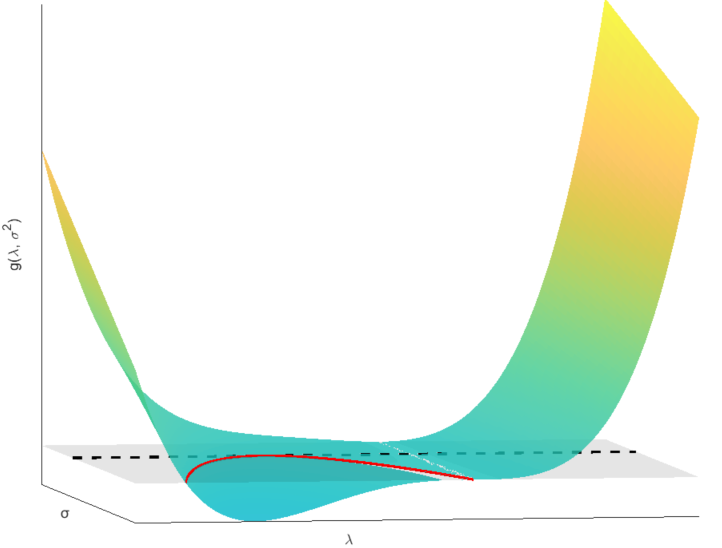
\includegraphics[width=8cm]{g_plot_p1p2-1325.png}
\caption{Numeric plots of $g_{\sigma,p}$ function for fixed $p=(0.13, 0.25)$ varying $\lambda$  and $\sigma^2$ from variance to upper bound $\sigma_{up}$}
\label{241029160153}
\end{figure}

%\textcolor{red}{We should add some plots of the function $g_{\sigma,p}$ for some given values of $(p_1,p_2)$ with varying $\sigma^2$ from the upper bound down to the variance. It is first convex, then now longer convex but with no oscillation and then starts oscillating until it reaches the optimal value. When we hit the variance, it becomes obviously negative locally around $0_-$.}

\subsubsection{The case $p_3>4\sqrt{p_1p_2}$}
In this case, we have $\Delta>0$ and $P$ has two distinct positive roots $0<X_-<X_+$ so that $N_{p_1,p_2}$ has exactly two roots $\lambda_-<\lambda_+$. Their location is given by the following lemma.

\newtheorem*{manuallemma}{Lemma 1.1}
\begin{manuallemma}
\label{lemma:lambda_ordering}
Let $p_1, p_2 \in \mathbb{R}$ such that $p_2 \geq p_1$ and $p_3^2>16p_1p_2$. Then the following inequality holds:
\[
\lambda_0 \leq 0 <\lambda_- <   \lambda_+
\]
\end{manuallemma}
\begin{proof}Let us first observe that we have:
\bea \lambda_{-}= \ln\left(\frac{p_3^2-8p_1p_2 - \sqrt{(p_3^2-4p_1p_2)(p_3^2-16p_1p_2)}}{2p_1p_2}\right) \cr \lambda_{+} =\ln\left(\frac{p_3^2-8p_1p_2 +  \sqrt{(p_3^2-4p_1p_2)(p_3^2-16p_1p_2)}}{2p_1p_2}\right) \eea
%we have $\sqrt{(p_3^2-4p_1p_2)(p_3^2-16p_1p_2)} > 0$ and $p_3^2-8p_1p_2 > 8p_1p_2$ thus  $p_3^2-8p_1p_2 +  \sqrt{(p_3^2-4p_1p_2)(p_3^2-16p_1p_2)} > 8p_1p_2$ thus $\lambda_+>\ln(4)$ and as $\lambda_0 \leq 0$ we conclude $\lambda_+>\lambda_0$\\
We shall denote for compactness $x := p_3^2>0$, $y := p_1p_2>0$ so that we have the condition $x>16y$. Since $\lambda_0<0$, we only need to prove that $\lambda_->0$. We will now prove that $\lambda_{-} > 0$ under the condition $x > 16y>0$. To establish this result, we proceed through a chain of equivalent inequalities, beginning with the definition of $\lambda_{-}$
\begin{align*}
\lambda_{-} > 0 
&\iff \frac{x - 8y - \sqrt{(x-4y)(x-16y)}}{2y} > 1 \\
&\iff x - 8y - \sqrt{(x-4y)(x-16y)} > 2y \\
&\iff x - 10y > \sqrt{(x-4y)(x-16y)} \\
&\iff (x - 10y)^2 > (x-4y)(x-16y) \quad (\text{because } x > 16y \Rightarrow x-10y > 6y > 0) \\
&\iff x^2 - 20xy + 100y^2 > x^2 - 20xy + 64y^2 \\
&\iff 100y^2 > 64y^2 \\
&\iff 36y^2 > 0 \quad (\text{always valid for  } y \neq 0)
\end{align*}
Thus we get  $\lambda_0 < 0 <\lambda_- <   \lambda_+$ under the condition $p_3^2>16p_1p_2$ ending the proof of the lemma.  
\end{proof}
%\begin{proof}The proof is done by straightforward computations and inequalities and is presented in \autoref{AppendixLemma}.
%\end{proof}

We shall now use split the analysis of the sign of $g(.;\sigma^2)$ on $\mathbb{R}_-^*$ and $\mathbb{R}_+^*$. Let us first observe that the discussion made for $\mathbb{R}_-^*$ in the proof of \autoref{TheoRegime1} is still valid. Thus, $g(.;\sigma^2)$ is non-negative on $\mathbb{R}_-^*$ if and only if $\sigma^2\geq \frac{2(p_2-p_1)}{\ln \frac{p_2}{p_1}}$. Let us now discuss the situation on $\mathbb{R}_+^*$. From \autoref{lemma:lambda_ordering} and \eqref{g3} we get that $g^{(3)}$ is negative on $(-\infty,\lambda_0)\cup\left(\lambda_-(\sigma),\lambda_+(\sigma)\right)$  and positive on $(\lambda_0,\lambda_-(\sigma))\cup\left(\lambda_+(\sigma),+\infty\right)$. Consequently, $g''(.;\sigma^2)$ is increasing on $(0,\lambda_-)$ and since $g''(0;\sigma^2)=0$ is it thus positive on this interval. Then, $g''(.;\sigma^2)$ is decreasing on $(\lambda_-(\sigma),\lambda_+(\sigma))$ and then increasing on $(\lambda_+(\sigma),+\infty)$ with $g''(+\infty;\sigma^2)=\sigma^2>0$. Thus, there are only two possible cases: either $g''(\lambda_+(\sigma);\sigma^2)\geq 0$ and then $g(.;\sigma^2)$ is strictly convex and positive on $\mathbb{R}_+^*$ or $g''(\lambda_+(\sigma);\sigma^2)<0$ in which case $g''(.\sigma^2)$ has exactly two zeros $(\lambda_1(\sigma),\lambda_2(\sigma))$ on $\mathbb{R}_+^*$ such that $\lambda_-(\sigma)<\lambda_1(\sigma)<\lambda_+(\sigma)<\lambda_2(\sigma)$. We may thus apply \autoref{LemmaNumber} whose conclusion depends on the existence of a solution $(\lambda,\sigma^2)\in \left(\lambda_-,+\infty\right)*\times \left(\operatorname{Var}[Y],+\infty\right)$ of the equation $g(\lambda;\sigma^2)=0=g'(\lambda;\sigma^2)$. This set of equations is equivalent to
\beq \sigma^2=\frac{1}{\lambda}\left(\frac{u_1(\lambda)}{u_0(\lambda)}-\mu\right)=\frac{1}{\lambda}\left(p_1-p_2+\frac{p_2e^\lambda-p_1e^{-\lambda}}{p_1e^{-\lambda}+p_2e^{\lambda}+1-p_1-p_2}\right)
\eeq
and $\lambda$ positive solution of
\beq \lambda \frac{u_1(\lambda)}{u_0(\lambda)}- 2\ln (u_0(\lambda))+\lambda \mu=0\eeq
i.e.
\beq \label{EqF} F(\lambda):=\lambda u_1(\lambda)-2u_0(\lambda)\ln u_0(\lambda)+ \lambda u_0(\lambda)(p_2-p_1)=0\eeq
From \autoref{LemmaNumber2}, $F(\lambda)=0$ has no solution on $\mathbb{R}_+^*$ such that $\sigma^2=\frac{1}{\lambda}\left(\frac{u_1(\lambda)}{u_0(\lambda)}-\mu\right)<\operatorname{Var}[Y]$. Thus, we have two cases:
\begin{itemize}
    \item If $F$ has a positive zero $\lambda_c>0$ then \autoref{LemmaNumber} implies that this zero is unique on $\mathbb{R}_+^*$ and we get that $\sigma_c^2=\frac{1}{\lambda_c}\left(\frac{u_1(\lambda_c)}{u_0(\lambda_c)}-\mu\right)\geq\operatorname{Var}[Y]$. \autoref{GeneralCharac} implies that the optimal variance proxy is given by
    \beq \sigma_{\mathrm{opt}}^2=\max\left(\frac{2(p_2-p_1)}{\ln \frac{p_2}{p_1}}, \frac{1}{\lambda_c}\left(\frac{u_1(\lambda_c)}{u_0(\lambda_c)}-(p_2-p_1)\right) \right)\eeq
    \item If $F$ has no zero on $\mathbb{R}_+^*$ then $g(.;\sigma^2)$ is positive on $\mathbb{R}_+^*$ and thus the optimal variance proxy is given by $\sigma^2_{\text{opt}}=\frac{2(p_2-p_1)}{\ln \frac{p_2}{p_1}}$.
\end{itemize}

\begin{remark}Note that $\underset{\lambda\to +\infty}{\lim} F(\lambda)=-\infty$ and $F(\lambda)=\frac{1}{6}M_3[Y]\lambda^3+\frac{1}{4}\left(\frac{1}{3}M_4[Y]-\operatorname{Var}[Y]^2\right)\lambda^4+ O(\lambda^5)$, where $M_3:=\mathbb{E}[(Y-\mu)^3]$ and $M_4:=\mathbb{E}[(Y-\mu)^4]$. Thus, a sufficient condition for $F$ to admit a positive zero is that $M_3[Y]>0$ or $\left[M_3[Y]=0 \text{ and } \frac{1}{3}M_4[Y]\operatorname{Var}[Y]^2>0\right]$. In particular for $p_1=p_2=p$, we have that $F(\lambda)=\frac{1}{6}p(1-6p)\lambda^4+O(\lambda^5)$ so that for $p>\frac{1}{6}$ (which is the equivalent condition to $p_3>4\sqrt{p_1p_2}$ in this case) $F$ always has a unique positive zero $\lambda_c$ and the corresponding variance $\sigma_c^2=\frac{1}{\lambda_c}\frac{u_1(\lambda_c)}{u_0(\lambda_c)}$ is always greater than $2p=\operatorname{Var}[Y]$ and hence the optimal variance proxy is always $\sigma_{\mathrm{opt}}^2=\sigma_c^2=\frac{1}{\lambda_c}\frac{u_1(\lambda_c)}{u_0(\lambda_c)}$ in the symmetric case $p_1=p_2=p$.
\end{remark}


% \textcolor{red}{Olivier: There are cases where $F$ does not admit a positive zero. For example $(p_1,p_2)=(0.01, 0.5)$ which belongs to the second regime. }

% \medskip

% \textcolor{red}{To be done: General theorem tells us that the optimal variance proxy selects the biggest value of $\sigma^2$. However, apart from the symmetric case which is dealt with in the previous remark, it is not even clear that there is a positive zero of $F$ in the second regime. I have plots where the zero exists and some where it does not. Logically, there should also be cases for which the zero exists but the corresponding variance is not the biggest one. Therefore, at this stage it would be good to have a 3d plot of the optimal variance relatively to $(p_1,p_2)$. When $p_1+p_2=1/3$, we have $\sigma_c^2=\frac{2(p_2-p_1)}{\ln \frac{p_2}{p_1}}$ and the positive zero is $\lambda_c=\ln(p_2/p_1)>0$. This is a case where both critical variance are equal so this also possible even in the non-symmetric case.}

%\newpage
\section{Application to uniform discrete distributions}\label{sec:uniform}
Let \( X \) be a random variable with finite support defined as \(X(\Omega)=\{x_1, x_2, \ldots, x_N\}\), where $N>1$, and each point is equiprobable: 
\[
  \mathbb{P}(X = x_k) = \frac{1}{N}, \quad \text{for all } k \in \{1,2,\dots,N\}.
\]
We consider that the support points are regularly spaced, such that there exist parameters \( a \in \mathbb{R} \) and  \( h \in  \mathbb{R}^{*}_{+} \) satisfying
 \[
 x_k = ka  + h , \quad \ k = 1,2,\dots,N.
 \]
Introducing the normalized random variable
 \[
 Y = \frac{X-h}{a}
 \]
and employing the linearity property of the optimal variance proxy, we have the relation
\[
\sigma_{\mathrm{opt}}[X] = a\sigma_{\mathrm{opt}}[Y].
\]
Thus, without loss of generality, we can restrict our attention to the simplified case $a=1$ and $h=0$. Under this assumption, the variable $Y$ is uniformly distributed on the integer set $\{1, 2, \ldots, N\}$ , with the well-known moments:
\beq
  \mu:=\E[Y]=\frac{N+1}{2}, \quad  \sigma^2:=\operatorname{Var}[Y]=\frac{N^2-1}{12}, \quad \operatorname{\kappa_3}[Y] := \E[(Y-\E[Y])^3]=0.
\eeq
By definition, a real number $\sigma>0$ is said to be a \emph{variance proxy} of $Y$  if and only if it satisfies the following exponential inequality for all $\lambda \in \mathbb{R}$:
\beq
\E\left[e^{\lambda Y}\right]=  \frac{1}{N}\sum_{k=1}^{N} e^{\lambda k} \leq e^{\left(\frac{\lambda^2\sigma^2}{2}+\lambda \mu\right)} \,\, ,\,\, \forall \, \lambda\in \mathbb{R}.
\eeq
This condition can be equivalently rewritten as the non-negativity requirement on the function:
\beq
g_{\sigma,N}(\lambda):=\frac{\lambda^2\sigma^2}{2}-u(\lambda)+\lambda \frac{N+1}{2} \geq 0 \,\,,\,\,  \forall \, \lambda\in \mathbb{R}.
\eeq
Where we define the log-partition function as:
\[
u(\lambda) := \ln\left(\frac{1}{N}\sum_{k=1}^{N} e^{\lambda k}\right).
\]
By general theory, it follows that the variance $\operatorname{Var}[Y]=\frac{N^2-1}{12}$ provides a lower bound for the optimal variance proxy. Hence, in our analysis we consider $\sigma\geq \sqrt{\frac{N^2-1}{12}}$.\\

To characterize the optimal variance proxy, it is essential to study the properties of the function $g_{\sigma, N}$. Observe that $g_{\sigma, N}$ is a smooth function of $(\sigma, \lambda, N)$. Its first three derivatives with respect to $\lambda$ are explicitly computed as:
 
\begin{align*}
g'_{\sigma,N}(\lambda)   &= \lambda \sigma^2 - u'(\lambda) + \mu \\
g^{(2)}_{\sigma,N}(\lambda) &= \sigma^2 - u^{(2)}(\lambda)\\
g^{(3)}_{\sigma,N}(\lambda) &= - u^{(3)}(\lambda).
\end{align*}
To analyze the properties of the function \( u(\lambda) \), and consequently those of \( g_{\sigma,N}(\lambda) \), we introduce an auxiliary family of probability distributions. This approach allows us to leverage probabilistic tools to study the behavior of \( u(\lambda) \) and its derivatives.\\
Let \( \mathcal{I} = \{1, \ldots, N\} \). For every real number \( \lambda \), consider the family of probability distributions \( (P_\lambda)_{\lambda \in \mathbb{R}} \) on \( \mathcal{I} \) defined by
\beq
P_\lambda(k) = \frac{e^{\lambda k}}{\sum_{j=1}^N e^{\lambda j}}, \quad k \in \mathcal{I}.
\eeq
We denote by \( \mathbb{E}_\lambda[\cdot] \), \( \operatorname{Var}_\lambda[\cdot] \), and \( \operatorname{\kappa}_{3,\lambda[}\cdot] \) the expectation, variance and  third central moment with respect to \( P_\lambda \), respectively. Note that when \( \lambda = 0 \), this distribution reduces to the uniform distribution over \( \mathcal{I} \).
This family of distributions satisfies several fundamental identities, including symmetry properties and a moment derivative formula.
\paragraph{Symmetry identities.}
    \begin{itemize}
        \item \( P_{-\lambda}(k) = P_\lambda(N - k + 1) \),
        \item \( \mathbb{E}_{-\lambda}[Z] = N + 1 - \mathbb{E}_\lambda[Z] \),
        \item \( \operatorname{Var}_{-\lambda}[Z] = \operatorname{Var}_\lambda[Z] \).
    \end{itemize}
\paragraph{Moment derivative identity.} For all integers \( m \geq 1 \),
    \[
    \frac{d}{d\lambda} \mathbb{E}_\lambda[Z^m] = \mathbb{E}_\lambda[Z^{m+1}] - \mathbb{E}_\lambda[Z]\,\mathbb{E}_\lambda[Z^m].
    \]
These identities will be used repeatedly in the analysis of the log-partition function and its derivatives.
\begin{lemma}[Derivatives of log-partition function as moments]\label{lem:log_partition_moments}
The derivatives of \( u(\lambda) \) give the moments of the associated exponential family distribution:
\beq
u'(\lambda) = \mathbb{E}_{\lambda}[Z], \quad u^{(2)}(\lambda) = \operatorname{Var}_{\lambda}[Z], \quad u^{(3)}(\lambda) = \mathbb{E}_{\lambda}[(Z - \mathbb{E}_{\lambda}[Z])^3] = \operatorname{\kappa}_{3,\lambda}[Z]
\eeq
\end{lemma}

\begin{proof}
These identities follow directly from the moment derivative formula combined with the expressions for the first moments. Applying the derivative identity recursively yields the expressions for \( u'(\lambda) \), \( u^{(2)}(\lambda) \), and \( u^{(3)}(\lambda) \), which correspond to the mean, variance, and third centered moment under \( P_\lambda \).
\end{proof}

From Symmetry identities, we know that  $\operatorname{Var}_{\lambda}[X]$ is an even function of $\lambda$. This symmetry allows us to restrict our analysis to $\mathbb{R}_+$. Given the derivative relationship 
 \beq \operatorname{\kappa}_{3,\lambda}[Z] = \frac{d}{d\lambda}\operatorname{Var}_{\lambda}[Z] \eeq
along with the evenness of the variance, it follows that the the third central moment is an odd function of $\lambda$. Thus we can restrict our analysis to \( \mathbb{R}_+ \).

\begin{lemma}
[Negativity of the third derivative of the log-partition function]\label{lemma:neg_third_deriv}
Let \( N \geq 2 \) be an integer and let \( \lambda > 0 \) be a real number. Then the third derivative of the log-partition function is strictly negative. In other words,
\beq
u^{(3)}(\lambda) = -\frac{N^3 e^{\lambda N}(1 + e^{\lambda N})}{(1 - e^{\lambda N})^3} + \frac{e^{\lambda}(1 + e^{\lambda})}{(1 - e^{\lambda})^3} < 0, \quad \forall \lambda\in \mathbb{R}.
\eeq
Consequently,
\beq
\operatorname{\kappa}_{3,\lambda}[Z] < 0 \text{ for all } \lambda \in \mathbb{R}_+^*
\eeq
\end{lemma}
\begin{proof}
The explicit expression  of \( u^{(3)}\) follow by direct differentiation of \( u(\lambda) = \ln S(\lambda) \), where $ S(\lambda) = \frac{1}{N}\sum_{k=1}^N e^{\lambda k}$ and using the closed-form expression for the geometric sum.\\
Consider the auxiliary function
\[
f(t) = \frac{t(t + 1)}{(1 - t)^3}, \quad \text{for } t = e^{\lambda} > 1.
\]
We compute its derivative:
\[
f'(t) = \frac{1 + 4t + t^2}{(1 - t)^4}.
\]
Since both the numerator and the denominator are strictly positive for all \( t > 1 \), we conclude that \( f'(t) > 0 \). Hence, \( f \) is strictly increasing on the interval \( (1, \infty) \).

Now fix \( \lambda > 0 \), so that \( t = e^{\lambda} > 1 \). Since \( N \geq 2 \), we have \( t^N > t \). By the monotonicity of \( f \), it follows that
\[
f(t^N) > f(t),
\]
which yields the inequality
\[
\frac{e^{\lambda N}(1 + e^{\lambda N})}{(1 - e^{\lambda N})^3} > \frac{e^{\lambda}(1 + e^{\lambda})}{(1 - e^{\lambda})^3}.
\]

Furthermore, since \( N^3 \geq 8 \) for all \( N \geq 2 \), we obtain
\[
\frac{N^3 e^{\lambda N}(1 + e^{\lambda N})}{(1 - e^{\lambda N})^3} > \frac{e^{\lambda}(1 + e^{\lambda})}{(1 - e^{\lambda})^3}.
\]

Therefore, the third derivative of the log-partition function satisfies
\[
u^{(3)}(\lambda) 
= - \frac{N^3 e^{\lambda N}(1 + e^{\lambda N})}{(1 - e^{\lambda N})^3}
+ \frac{e^{\lambda}(1 + e^{\lambda})}{(1 - e^{\lambda})^3}
< 0,
\]
which completes the proof.
\end{proof}

\paragraph{Variance proxy optimality.}
Lemma~\ref{lemma:neg_third_deriv} shows that
\[
\kappa_{3,\lambda}[Z] = \frac{d}{d\lambda}\operatorname{Var}_{\lambda}[Z] < 0, \quad \forall \lambda > 0.
\]
As \( \operatorname{Var}_{\lambda}[Z] \) is an even function of \( \lambda \), it follows that it is strictly increasing on \( \mathbb{R}_- \), strictly decreasing on \( \mathbb{R}_+ \), and attains a unique global maximum at \( \lambda = 0 \). In particular,
\[
\operatorname{Var}_{\lambda}[Z] \leq \operatorname{Var}_0[Z] = \operatorname{Var}[Z], \quad \forall \lambda \in \mathbb{R}.
\]
Hence, for any \( \sigma^2 \geq \operatorname{Var}[Z] \), we have \( g_{\sigma,N}^{(2)}(\lambda) = \sigma^2 - \operatorname{Var}_\lambda[Z] \geq 0 \), with equality if and only if \( \lambda = 0 \). The system of equations
\[
g_{\sigma,N}(\lambda,\sigma^2) = 0, \quad \frac{\partial}{\partial \lambda} g_{\sigma,N}(\lambda,\sigma^2) = 0
\]
admits a unique solution at \( \lambda = 0 \), which is the global minimum of \( g_{\sigma,N}^{(2)} \). Moreover, since the third derivative \( g_{\sigma, N}^{(3)}(\lambda) \) is positive on \( \mathbb{R}_+ \) and negative on \( \mathbb{R}_- \), the function \( g_{\sigma, N}^{(2)}(\lambda) \) is strictly convex and minimized at \( \lambda = 0 \). This confirms that
\[
\sigma^2_{\mathrm{opt}}[Y] = \operatorname{Var}[Y] = \frac{N^2 - 1}{12}
\]
is the optimal variance proxy, and implies that \( Y \) is strictly sub-Gaussian.
% \newpage
% \section{Software implementation}\label{sec:software}


% \section{Discrete random variables}
% In this section, we study the optimal variance proxy for finite discrete K-ary random variables with bounded support $K \geq 3$. Their sub-Gaussianity are  ensured by classical Hoeffding's lemma:\\
% if \(X\)  is a random variable supported on $[a,b]$ with mean $\mu = \mathbb{E}(X)$, then for all $\lambda \in \mathbb{R}$
% \begin{equation}
%     \mathbb{E}\left[\exp({\lambda (X - \mu))}\right] \leq \exp\left(\frac{\lambda^2 (b-a)^2}{8}\right)
%         \label{eq:hoeffdings_lemma}
% \end{equation}
% This result guarantees that bounded random variables exhibit sub-Gaussian behavior, which is crucial for variance proxy analysis.
% \subsection{Sub-Gaussianity of binary variables}
% \cite{Kearns1998LargeDM} Lemma 1 showed that any binary random variable with mean $\mu$  is $\frac{1}{2g(\mu)}$-sub-gaussian :
% \begin{equation}
%     \mathbb{E}\left[e^{({\lambda (X - \mu))}}\right] \leq \exp\left(\frac{\lambda^2}{4g(\mu)}\right) \text{ for all } \lambda \in \mathbb{R}.
%     \label{eq:Kearns_lemma}
% \end{equation}
% where 
% \begin{equation}
%     g(\mu) = \frac{1}{1-2\mu}{\ln\frac{1-\mu}{\mu}}
% \end{equation}
% The sub-Gaussian property (\ref{eq:Kearns_lemma}) refines Hoeffding's inequality (\ref{eq:hoeffdings_lemma}) by introducing the mean-dependent term $g(\mu)$. For the Bernoulli distribution with mean $\mu \in (0,1)$,  \cite{buldygin2013sub} Theorem 2.1 established that $\frac{1}{2g(\mu)} $ constitutes the optimal variance proxy. This result was verified by \cite{marchal2017sub} Theorem 2.\\
% \textbf{Remark 1}. \textit{The variance proxy $\frac{1}{2g(\mu)}$ is distribution sensitive, for $\mu \rightarrow 0 \text{ or 1, we have }\\ g(\mu) \rightarrow +\infty \text{ reflecting lighter tails.}$}\\
% Henceforth, we denote $\underline{\textbf{a}} = (a_1, a_2, ..., a_K)$ and $\underline{\textbf{p}} = (p_1, p_2, ..., p_K)$

% \newpage
% \section*{Technical Results}

% \paragraph{Acknowledgment.}
% % ----------------------------------------------------------------
% We would like to thank ...
\bibliographystyle{plainnat}
\bibliography{references}


\appendix
\end{document}
